\documentclass[12pt]{article}
\usepackage{amsmath,amsfonts,amssymb,
        graphicx,hyperref,amsthm,subfig,authblk}
\usepackage[iso,american]{isodate}
\usepackage [margin=1in]{geometry}
\usepackage{enumerate}
\usepackage{listings}

% \usepackage{endnotes}
\usepackage{multirow}
% \doublespacing
\hypersetup{pdfborder={0 0 0}, colorlinks=true, urlcolor=black, linkcolor=blue}

% math shortcuts
\newcommand{\iid}{\stackrel{\mathrm{iid}}{\sim}}
\newcommand{\E}{\mathbb{E}}

% tikz stuff
\usepackage{pgf, tikz}
\usetikzlibrary{arrows, automata}


\begin{document}

\title{Modeling Predator Preferences}
\author{Edward A. Roualdes and Simon Bonner \\ University of Kentucky}
\date{\today}
\maketitle

\begin{abstract}
The literature on modeling a predator's prey selection includes many intuitive indices, few of which have both reasonable statistical justification and tractable asymptotic properties.  Here, we provide a simple model that meets both of these criteria, while extending previous work to include an array of multiple species and time points.  Further, we apply the Expectation-Maximization algorithm to cases where exact counts of the number of prey species eaten in a particular timer period is not observed.  A simulation is provided to demonstrate the accuracy of our methods.
\end{abstract}

\section{Introduction}
\label{sec:intro}

Modeling a predator's food selection was given much attention for a short period of time; see \citet{Strauss:1979} and the references within.  Many, if not all, of the indices developed, though intuitive, focused on a snapshot in time and only on one prey species, and they rarely had practicle asymptotic properties.  This has left interested practicioners to the most computationally manageable of the techniques, and has completely ignored simultaneous testing across an array of both species and time.

The model presented here, maintains tractable asymptotic properties while being general enough to take into account an array of speices and time points.  By modeling both time and any number of prey species, we are able to see a more detailed anlyais of the predator's eating preferences.  Further, the simplicity of the model allows us to consider predators for which exact tallies of the number of each variety of prey species eaten within any given time period is not observed.  Instead, we rely on the researcher being able to DNA sequence the contents of the predator's gut, and make a simple binary conclusion: yes this predator ate some of that prey species during this time period, or no they did not.  Under certain situations, our models is able to accurately estimate parameters of interest despite having lost much information.  

To showcase our model, we performed simulations for both scenarios when full count data from the predators' guts are observed, and when instead only binary repsonses, indicating specific prey species were eaten, are observed.  Our \texttt{R} \citep{R:2014} package, named \texttt{spiders}, is available on CRAN so that the broader community of researchers can similarly apply our methods.

%%% Local Variables: 
%%% mode: latex
%%% TeX-master: "main"
%%% End: 

\section{Methods}
\label{sec:methods}

\subsection{Data}

We assume data are collected in the following manner.  Traps are dispersed, for $T$ time periods, throughout the habitat of the predator and prey of interest.  Prey species, indexed by $s \in \{1, \ldots, S \}$, are collected in the traps and counted at each time period.  We assume these counts represent the number of prey species $s$ the predator will encounter on average during time period $t \in \{1, \ldots, T\}$.  The counts of prey species $s$ caught during time period $t$ are hypothesized to be independent draws from a Poisson distribution with rate parameter $\gamma_{st}$.  We further assume that the number of prey species found in the gut of the trapped predators, also follows a Poisson distribution with rate $\lambda_{st}$.  Here, the parameter $\lambda_{st}$ represents the rate at which the predator ate the encountered prey species $s$ during time period $t$.  By modeling $\lambda_{st}$ and $\gamma_{st}$ we are able to test claims about a predator's eating preferences.  

The use of Poisson distributions make the following implicit assumptions: $1)$ traps independently catch the prey species of interest, $2)$ predators eat, at a constant rate, prey species independently, $3)$ predators eat indepedent of each other.  Our model's ability to accurately portray predators' habitats and underlying eating preferences dependes on the degree to which these assumptions are broken.

Let $X_{jst} \iid \mathcal{P}(\lambda_{st})$ denote the number of prey species $s$ that predator $j$ ate during occurrence $t$ where $j \in \{1, \ldots, J_t\}$.  Let $Y_{ist} \iid \mathcal{P}(\gamma_{st})$ denote the number of prey species $s$ found in trap $i$ during occurrence $t$, $i \in \{1, \ldots, I_t\}$.  Formal statistical statements about the relative magnitudes of the parameters $\boldsymbol{\lambda}$ and $\boldsymbol{\gamma}$ offer insights to the relative rates at which predators eat particular prey species.  

% \begin{figure}
%   \centering
%   \begin{tabular}{rrcc}
%     & & \multicolumn{2}{c}{Time} \\
%     & & constant & varies \\
%     \cline{3-4}
%     \multirow{2}{*}{Species} & \multicolumn{1}{r|}{constant} & \multicolumn{1}{c}{$c$} & \multicolumn{1}{|c|}{$c_t$} \\ 
%     \cline{3-4}
%     & \multicolumn{1}{r|}{varies} & \multicolumn{1}{c}{$c_s$} & \multicolumn{1}{|c|}{$c_{st}$} \\
%     \cline{3-4}
%   \end{tabular}
%   \caption{The four hypotheses considered are shown by their symbolic representations, highlighting which indices are allowed to vary.  This is essentially the range of the mapping $\xi$.  }
%   \label{tab:hyp}
% \end{figure}

We consider five variations on the relative magnitude of $\lambda_{st}/\gamma_{st} = c_{st}$.  These five hypotheses each allow $c_{st}$ to vary by time, prey species, both, or neither.  Because the five hypotheses are nested, a natural testing order is suggested in Figure~\ref{fig:hier}.

\begin{enumerate}
\item $c_{st} = 1, s = 1, \ldots, S; t = 1, \ldots, T$
\item $c_{st} = c, s = 1, \ldots, S; t = 1, \ldots, T$
\item $c_{st} = c_s, s = 1, \ldots, S$
\item $c_{st} = c_t, t = 1, \ldots, T$
\item $c_{st} = c_{st}, s = 1, \ldots, S; t = 1, \ldots, T$
\end{enumerate}

\begin{figure}
  \centering
  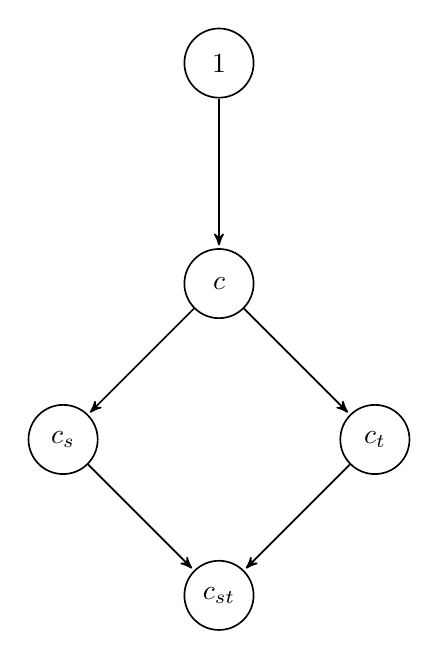
\begin{tikzpicture}[->,>=stealth',shorten >=1pt,auto,node distance=2.8cm, semithick]

    \node[state] (A)                    {$1$};
    \node[state] (B) [below of=A]       {$c$};
    \node[state] (C) [below left of=B]  {$c_s$};
    \node[state] (D) [below right of=B] {$c_t$};
    \node[state] (E) [below left of=D]  {$c_{st}$};

    \path       (A) edge node {} (B)
                (B) edge node {} (C)
                    edge node {} (D)
                (C) edge node {} (E)
                (D) edge node {} (E);
  \end{tikzpicture}
  
  \caption{Hierarchy of hypotheses.}
  \label{fig:hier}
\end{figure}

\subsection{Fully Observed Data}

The likelihood function that allows for estimation of these parameters is as follows.  Since we assume $X_{jst}$ is independent of $Y_{ist}$ we can simply multiply the respective Poisson probability density functions together, and then form products over all $s,t$ to get the likelihood.  

\begin{equation}
  \label{eq:likelihood}
  L(x_{jst}, y_{ist} |\boldsymbol{\lambda}, \boldsymbol{\gamma}) = \prod_{t = 1}^{T} \prod_{s=1}^S \left\{ \prod_{j=1}^{J_t} f_X(x_{jst}|\boldsymbol{\lambda}) \prod_{i=1}^{I_t} f_Y(y_{ist} | \boldsymbol{\gamma}) \right\}.
\end{equation}

\noindent Writing all $5$ hypotheses as $\lambda_{st} = c_{st}\gamma_{st}$, we can, in some cases find analytic solutions for the maximum likelihood estimates of $c_{st}$ and $\gamma_{st}$.  When the data are balanced $J_t = J$, $I_t = I$, and $c_{st} = c$ analytic solutions exist -- {\color{red}what about $c_{st} = 1$}.  In all other cases, analytic solutions are not readily available and instead we rely on the fact that the log-likelihood $l(\boldsymbol{\lambda}, \boldsymbol{\gamma}) = \log{L}$ is concave.  We maximize the log-likelihood by iteratively solving partial derivatives of $l$, with respect to $c_{st}$ and $\gamma_{st}$, set equal to zero

\begin{equation*}
  \hat{c} = \frac{\sum_{s,t} X_{\cdot st}}{\sum_t J_t \sum_s \gamma_{st}}, \quad \hat{c}_t =  \frac{\sum_s X_{\cdot st}}{J_t \sum_s \gamma_{st}}, \text{ or} \quad \hat{c}_s = \frac{\sum_{t}X_{\cdot st}}{\sum_t J_t \gamma_{st}}, \text{ and } \quad \hat{\gamma}_{st} = \frac{X_{\cdot st} + Y_{\cdot st}}{J_t c_{st} + I_t}.
\end{equation*}

\noindent where $X_{\cdot st} = \sum_{j=1}^{J_t}X_{jst}$ and $Y_{\cdot st} = \sum_{i=1}^{I_t} Y_{ist}$.


\subsection{Unobserved Counts}

Working with biologists who study spider eating preferences, we have found that not all predators' allow for easily counted prey species in their guts.  As an alternative strategy, we can rely on the DNA sequencing of a sample from the predators' guts.  If such sequencing returns a positive response, say a $1$ if a particular predator ate prey species $s$ and $0$ otherwise, we can, albeit with some information lost, model predators' eating preferences with the above framework using the EM algorithm.  

When the data $X_{jst}$ are not observed, and instead a boolean response indicating if a predator ate any number of prey species $s$ during time $t$ is observed, we can still, to some degree, estimates the parameters of interest $\boldsymbol{\lambda}, \boldsymbol{\gamma}$.  Because some information is observed, we can treat the counts as missing and use the EM algorithm to find the maximum likelihood estimates of the observed data likelihood.  

We denote the binary response that the predator did in fact eat at least one prey species $s$ in time period $t$ by $Z_{jst} = 1(X_{jst} > 0)$.  Now, the observed data are independent and identically distributed Bernoulli observations with parameter $p_{st} = 1-\exp\{-\lambda_{st}\}$.  Using this we can find the complete data likelihood by first noting that the conditional distribution of the unobserved data $X_{jst}$ given $Z_{jst}, Y_{ist}, \boldsymbol{\lambda}, \boldsymbol{\gamma}$ is a truncated Poisson distribution

\begin{equation*}
  f_{X|Y,Z,\boldsymbol{\lambda},\boldsymbol{\gamma}}(x_{jst}) =
  \frac{\exp{\{-\lambda_{st}\}} \lambda_{st}^{x_{jst}}}{(1 - \exp{\{-\lambda_{st}\}}) x_{jst}!}1(x_{jst} > 0) \quad \text{ where } \quad \E_{[X|Y,Z]}X_{jst} = \frac{\lambda_{st} \exp{\{\lambda_{st} \}}}{\exp{\{ \lambda_{st} \}} - 1}.
\end{equation*}

\noindent From this conditional distribution we get the joint distribution of $X_{jst}, Z_{jst}$

\begin{equation*}
    f_{X,Z|\boldsymbol{\lambda}}(x_{jst},z_{jst}) = \left\{
    \begin{array}{lr}
      \exp{\{ -\lambda_{st} \}}, & x_{jst}=0 \mbox{ and } Z_{jst} = 0 \\
      \frac{\exp{\{-\lambda_{st} \}} \lambda_{st}^{x_{jst}}}{x_{jst}!}, & x_{jst} > 0 \mbox{ and } Z_{jst} = 1\\
      0 & \mbox{otherwise}
    \end{array}
  \right.
\end{equation*}

\noindent The E-step of the EM algorithm is completed by computing the expected value of the complete data log-likelihood with respect to $f_{X|Y,Z,\boldsymbol{\lambda},\boldsymbol{\gamma}}(x_{jst})$ to get

\begin{align*}
  \E l_{comp} 
  & = \E \log{f_{X,Z|\boldsymbol{\lambda}}(X_{jst},z_{jst})} + \log{f_{Y|\boldsymbol{\gamma}}(y_{ist})} \\
  & = \sum_{s=1}^S \sum_{t=1}^T \sum_{j=1}^{J_t} \E \log{f_{X,Z|\boldsymbol{\lambda}}(X_{jst},z_{jst})}
  + \sum_{s=1}^S \sum_{t=1}^T \sum_{i=1}^{I_t} \log{f_{Y|\boldsymbol{\gamma}}(y)} \\
  & = \sum_{s,t,j} \left( - \lambda_{st} 
    + z_{jst} \E X_{jst} \log{\lambda_{st}}  \right) + \sum_{s,t} \left( -I_t \gamma_{st} + Y_{\cdot st} \log{I_t \gamma_{st}} \right) + \text{const} \\
  & = \sum_{s,t} \left( -J_t \lambda_{st} + z_{\cdot st} \E X_{jst} \log{\lambda_{st}} \right) + \sum_{s,t} \left( -I_t \gamma_{st} + Y_{\cdot st} \log{I_t \gamma_{st}} \right) + \text{const}.
\end{align*}

The EM algorithm requires iteratively solving $(\boldsymbol{\lambda}^{(k+1)},\boldsymbol{\gamma}^{(k+1)}) = \argmax_{\boldsymbol{\lambda},\boldsymbol{\gamma}} \E l_{comp}^k$.  Though no analytic solution to this maximization exists, one idea is to iteratively solve partial derivatives of $\E l_{comp}$ set equal to zero until convergence.  In fact, as we only need find parameter values that increase the observed likelihood, we forgo fully iterating to find the maximum values of the parameters and instead perform just one step uphill within each EM iteration.  This strategy is significantly less computationally intensive, thus generating a much faster generalized EM (GEM) algorithm.  

This GEM algorithm accurately estimates the parameters when values of $\lambda_{st}$ are relatively small, such that zeros are prevalent in the data $Z_{jst}$.  In this case, not too much information is lost since estimation of $\E Z_{jst}$ can be estimated well by the proportion of observed zeros.  On the other hand, if the predator consistently eats a given prey species, few to no zeros will show up in the observed data and $\E Z_{jst}$ is estimated to be nearly $1$.  The loss of information is best seen by attempting to solve for $\lambda_{st}$ in the equation $1 = \E Z_{jst} = 1 - \exp\{-\lambda_{st}\}$; essentially $\lambda_{st}$ is sent off to $+\infty$. 

\subsection{Testing}

All hypotheses are evaluated via a likelihood ratio test (LRT), with statistic

\begin{equation*}
  \label{eq:LRT}
    \Lambda(X,Y) := -2 \log{ \frac{ \sup L(\theta_0|X,Y)}{ \sup L(\theta_1|X,Y)} },
\end{equation*}

\noindent where $\theta_0, \theta_1$ represent the parameters estimated under the null and alternative hypotheses, respectively.  It is well known that the asymptotic distribution of $\Lambda$ is a $\chi_{\rho}^2$ distribution with $\rho$ degrees of freedom.  Under the EM algorithm we use $L_{obs}(Z,Y)$ as the likelihood in the calculation of $\Lambda$.  

The degrees of freedom $\rho$ are set equal to the number of free parameters available in the stated hypotheses under question.  If we put the null hypothesis to be $H_0: \lambda_t = c_t \gamma_t$, for all $t$ and contrast this against $H_1: \lambda_{st} = c_{st}\gamma_{st}$ then there are $\rho = 2(S \cdot T) - S \cdot T - T = S \cdot T - T$ degrees of freedom.

A set of hypotheses is determined by the p-value of the $\chi^2_{\rho}$ distribution.  Hence, with a level of significance, $\alpha$, the null hypothesis is rejected in favor of the alternative hypothesis if $\mathbb{P}(\chi^2_{\rho} > \Lambda) < \alpha$.  

\subsection{Testing $c_{st}$}

After determining which model best fits the data, more detail can be extracted through a hypothesis test on the elements of $c_{st}$, or in vector notation as $\mathbf{c} \in \mathbb{R}^{S\cdot T}$.  Let the elements of $\hat{\mathbf{c}}$ be the estimated values, $\hat{c}_{st}$, as estimated via the above maximum likelihood framework.  Since $\hat{\mathbf{c}}$ is asymptotically normally distributed, any linear combination of the elements is also asymptotically normally distributed.  For instance, let $a$ be a vector of the same dimension of $\hat{\mathbf{c}}$.  Then $a^t\hat{\mathbf{c}}$ is asymptotically distrbuted as $\mathcal{N}(a^t\mathbf{c}, a^t\Sigma a)$, where $\Sigma$ is the covariance matrix of the asymptotic distrbution of $\hat{\mathbf{c}}$.  

Suppose, for example, that the hypothesis $c_s$ is determined to best fit the data with $s$ ranging $s = 1, 2$.  We can test to see whether or not the two species $s_1$ and $s_2$ are statistically equally preferred under the null hypothesis $\hat{c}_{s_1} = \hat{c}_{s_2}$.  This hypothesis is alternatively written in vector notation as $a^t\hat{\mathbf{c}} = 0$, where $a = (1, -1)^t$.  Tests of the following form $H_0: a^t\mathbf{c} = \mu$ against any alternative of interest are then standard $Z$-tests.  Similarly, confidence intervals of any level can be obtained if desired. 

%%% Local Variables: 
%%% mode: latex
%%% TeX-master: "main"
%%% End: 

\section{Simulations}
\label{sec:sim}

% use language like: data generating model and fitted model, not hypotheses

Our simulations assume two prey species and five time points, throughout.  Of the hierarchy of hypotheses, we generate data under three models: $c, c_s, c_t$.  Sample sizes for both prey species and predator gut count observations are randomly chosen from four overlapping levels.  Let ``small'' sample sizes be randomly sampled numbers in $[20,50]$, ``medium'' encompass $[30,75]$, ``large'' $[50,150]$, and ``huge'' $[100,200]$.  Hence, we randomly sample for each time period from one of the sample size levels, then generate data for all models.  This is repeated for each level of sample size.  We simulate $500$ replicate datasets for each of the twelve scenarios above for both types of data, fully observed count data, $X_{jst}$, and for non-count data, when we observe only a binary response, $Z_{jst} = 1(X_{jst}>0)$.  Each scenario is then fit with the true model that generated the data.  All simulations of non-count data use $\tau = 10^{-5}$ as the convergence tolerance.  A subset of the examples are provided here; the interested reader is referred to the supplementary materials for the complete set of simulation results.

For all simulated data, the true parameter values for the rate at which prey species are encountered in the wild are fixed to be $\gamma_{st} = \pi, \, \forall s,t$. The values of $\lambda_{st}$ are set with respect to each data generating model.  For the model $c_{st} = c$, where predator preferences don't vary by either time or species, we consider $\lambda_{st} = 2\pi, \forall s,t$.  Under the model $c_s$, the ratio of rates vary by species only, so we put $\lambda_{1t} = \sqrt{2}$ and $\lambda_{2t} = \pi$.  Hence, $c_1 = \sqrt{2}/\pi \approx 0.45$ and $c_2 = 1$.  For the last model, $c_t$, the ratio of rates vary by time $t$.  Here, we put $\lambda_{st} = t$ for $t \in \{1, \ldots, 5 \}$.  

\begin{figure}
  \centering
  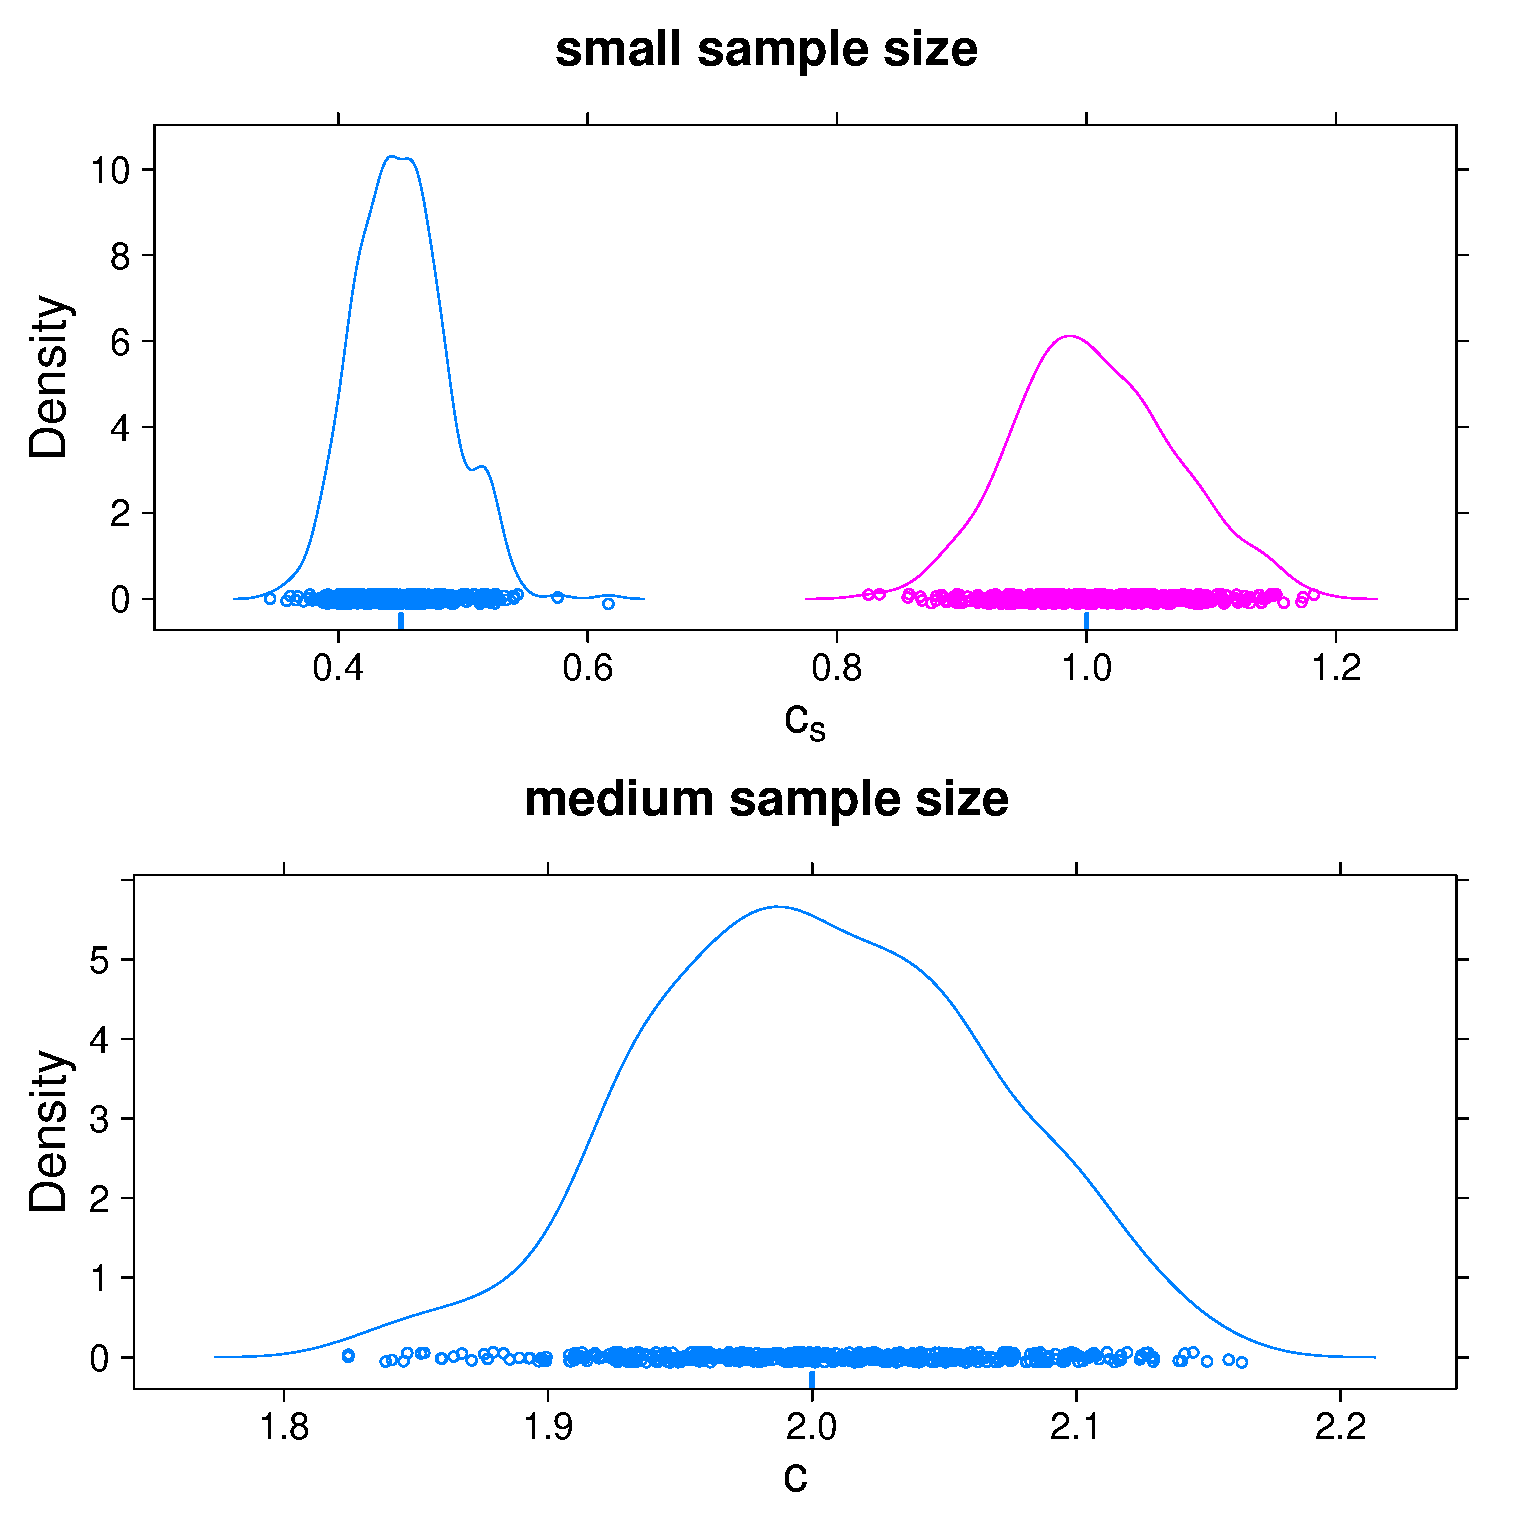
\includegraphics[scale=0.5]{nonem}
  \caption{Density plots of all $500$ estimates of fitting the true model to the data generated from models $c_s,c$ are shown with sample sizes small and medium, repsepectively.}
  \label{fig:nonem}
\end{figure}

% more words about how these numbers were estimated; estimtes from across all simulations
% simulations show nearly unbiased
% drop decimal places; we don't have precision to state further. 2

Figure~\ref{fig:nonem} shows density plots of the estimates of $c_s, c$ when fitting the true model to the fully observed count data generated under models $c_s$ and $c$.  The plots provide evaluations of parameter bias under each scenario.  In the first display, the parameters $c_1 \approx 0.45$ and $c_2 = 1$ are on average, across all $500$ simulations, estimated as $\hat{c}_1 = 0.45$ and $\hat{c}_2 = 1.00$, with standard errors of $\text{se}(\hat{c}_1) = 0.03$ and $\text{se}(\hat{c}_2) = 0.06$.  The second display provides a similar conclusion.  Averaging across all $500$ simulations, the parameter $c=2$ is estimated as $\hat{c} = 2.00$.  This is further seen in figure~\ref{fig:bp}, where box plots of the parameter estimates, centered at true parameter values, of the correct model fit to data generated from both $c_s$ and $c_t$ show empirically almost no bias.

\begin{figure}
  \centering
  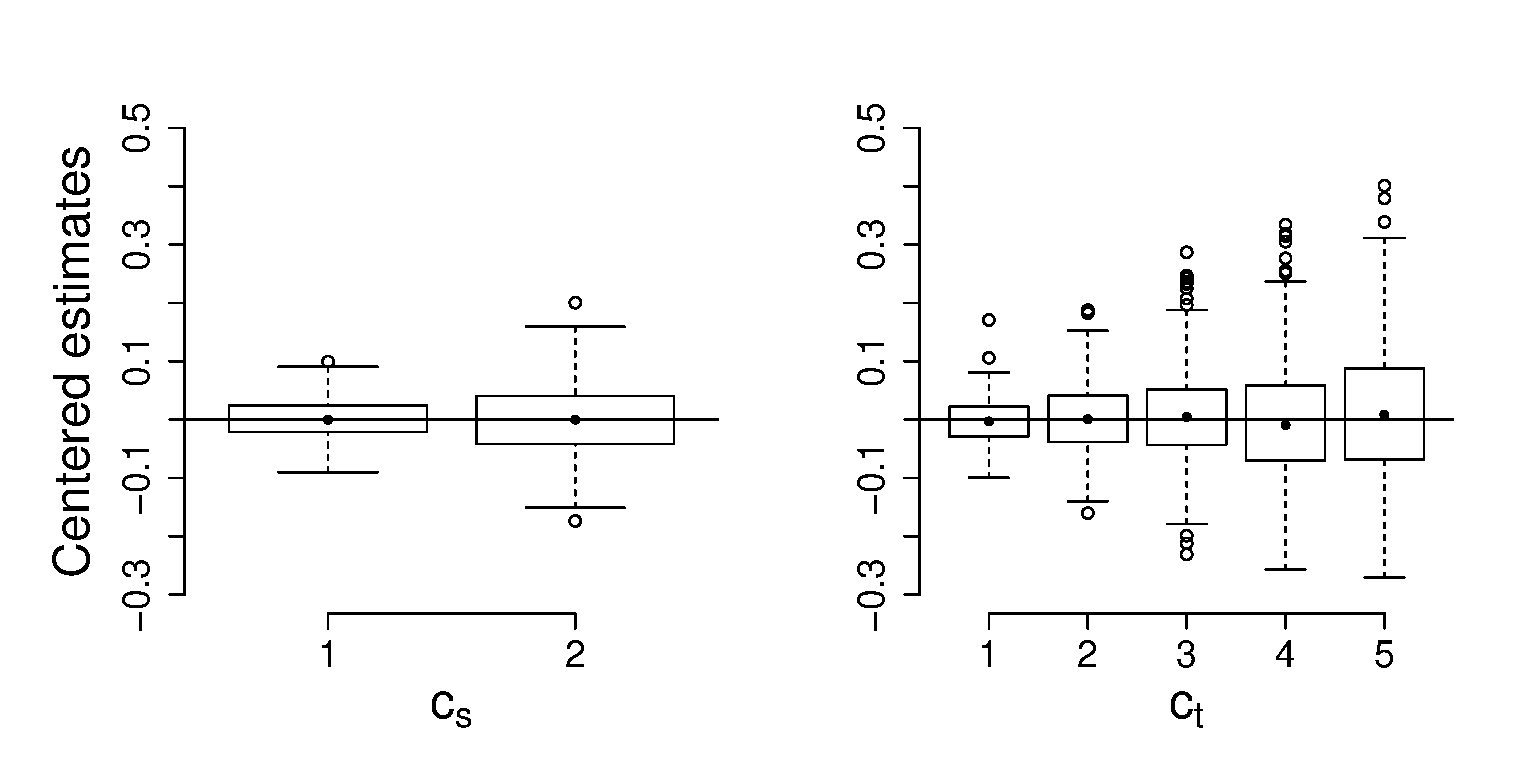
\includegraphics[scale=0.5]{bp}
  \caption{Shown are all $500$ estimates, centered at the true parameter values, from fitting the true model to the data generated from models $c_s,c$ with sample sizes small and medium, repsepectively.}
  \label{fig:bp}
\end{figure}

When we generate data with unobserved counts, the story is slightly different.  As noted above under certain circumstatnces our EM model accurately estimates the parameters of interest, and at different times can greatly over-estimate the parameters.  To investigate this issue further, we consider the same scenarios mentioned above, but now we reduce all of our count data down to binary observations.  For each scenario's generated data, we fit our EM algorithm as if we knew a priori the true underlying model that generated the observed data.

Figure~\ref{fig:em} contains density plots of fitting the true model, for all $500$ replications, of the data generating models $c_s,c_t$ with small and huge sample sizes, respectively.  When data are generated under the model $c_s$ and the true model fit to the non-count data, we find even for the small sample size that point estimates are reasonable.  When parameter values are of sufficient size to make zeros in the simulated data less common, the estimates from fitting the correct model to the generated data are occassionally over-estimated.  This effect is easily seen in figure~\ref{fig:em} for larger values of $c_t$ despite the increased sample size, but is also seen, less dramatically, in the density plot for the $c_s$ generated data.  

The seemingly arbitrary clustering of estimates near four seen in figure~\ref{fig:em} is due to two competing factors.  As the proportion of ones in the $Z_{jst}$ observations increases, the observed log-likelihood becomes flatter.  Thus, any finite convergence tolerance will cause the algorithm to terminate eventually.  By decreasing $\tau$, and increasing, as appropriate, the maximum iterations allowed within the EM algorithm, one can gradually increase the magnitude of a maximum likelihood estimate.

% The plots of $\gamma_{st}$ under the EM algorithm are not given as we do not consider missing data in the estimation of these parameters. 

% more of which model are we fitting, which model is generating the data

\begin{figure}
  \centering
  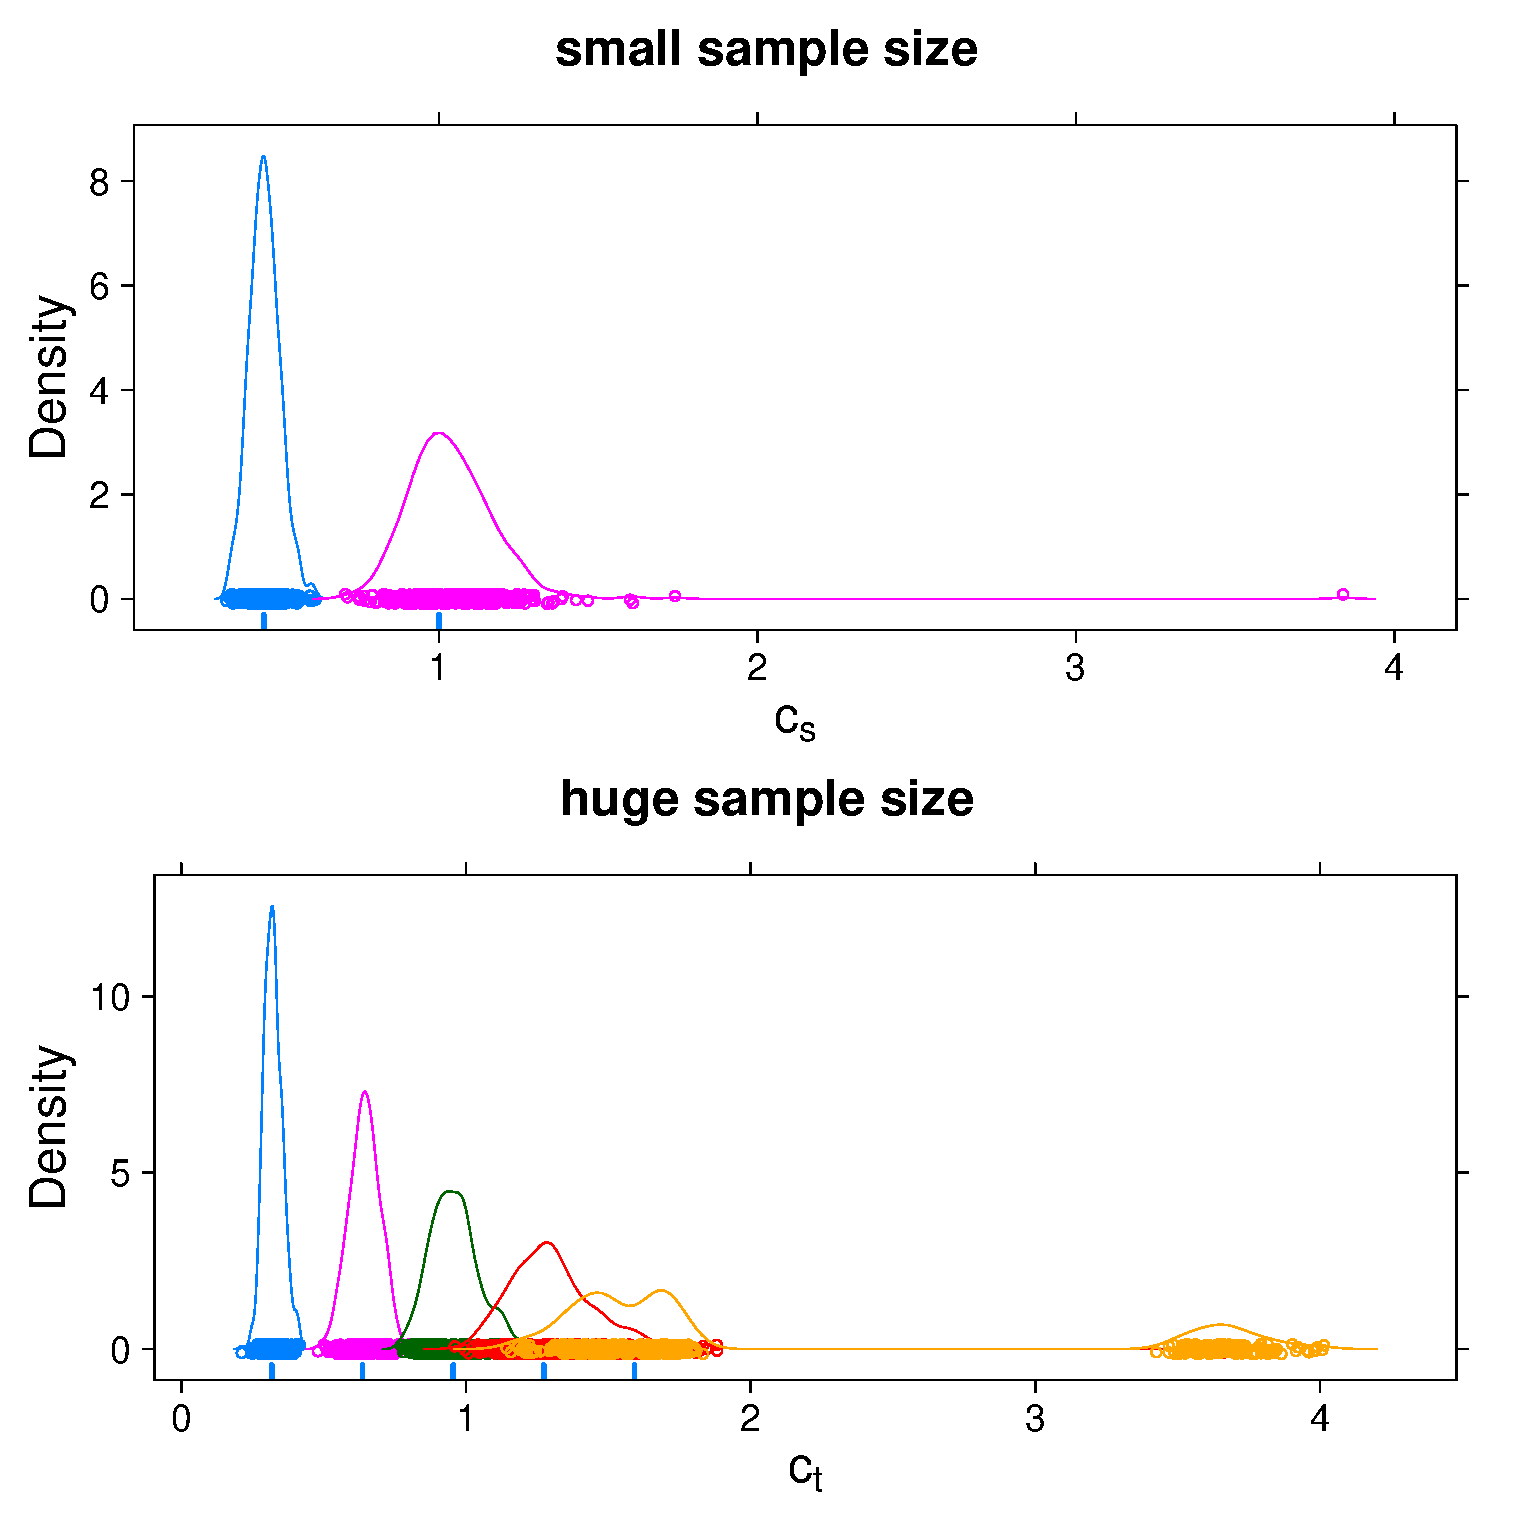
\includegraphics[scale=0.5]{em}
  \caption{Density plots of all $500$ estimates of fitting the true model to the data generated from models $c_s,c_t$, when counts are not observed, are shown with sample sizes small and huge, repsepectively.}
  \label{fig:em}
\end{figure}

The over-estimation of parameters, a symptom of the loss of information due to the unobserved counts, can also be seen with box plots of the $500$ point estimates, centered at their respective true parameter values.  Figure~\ref{fig:em_bp} contains box plots of the same scenarios in Figure~\ref{fig:em}, but with the small and huge sample sizes.  It is clear that as the parameters values increase and zeros in the observed data $Z_{jst}$ become less prevalent, over-estimation occurs more frequently.  This over-estimation, when it occurs, will generally increase the magnitude of the bias.

%Table~\ref{tab:bias} displays the max absolute bias across all indices $s,t$ of $\lambda_{st}$ for each simulation scenario.


\begin{figure}
  \centering
  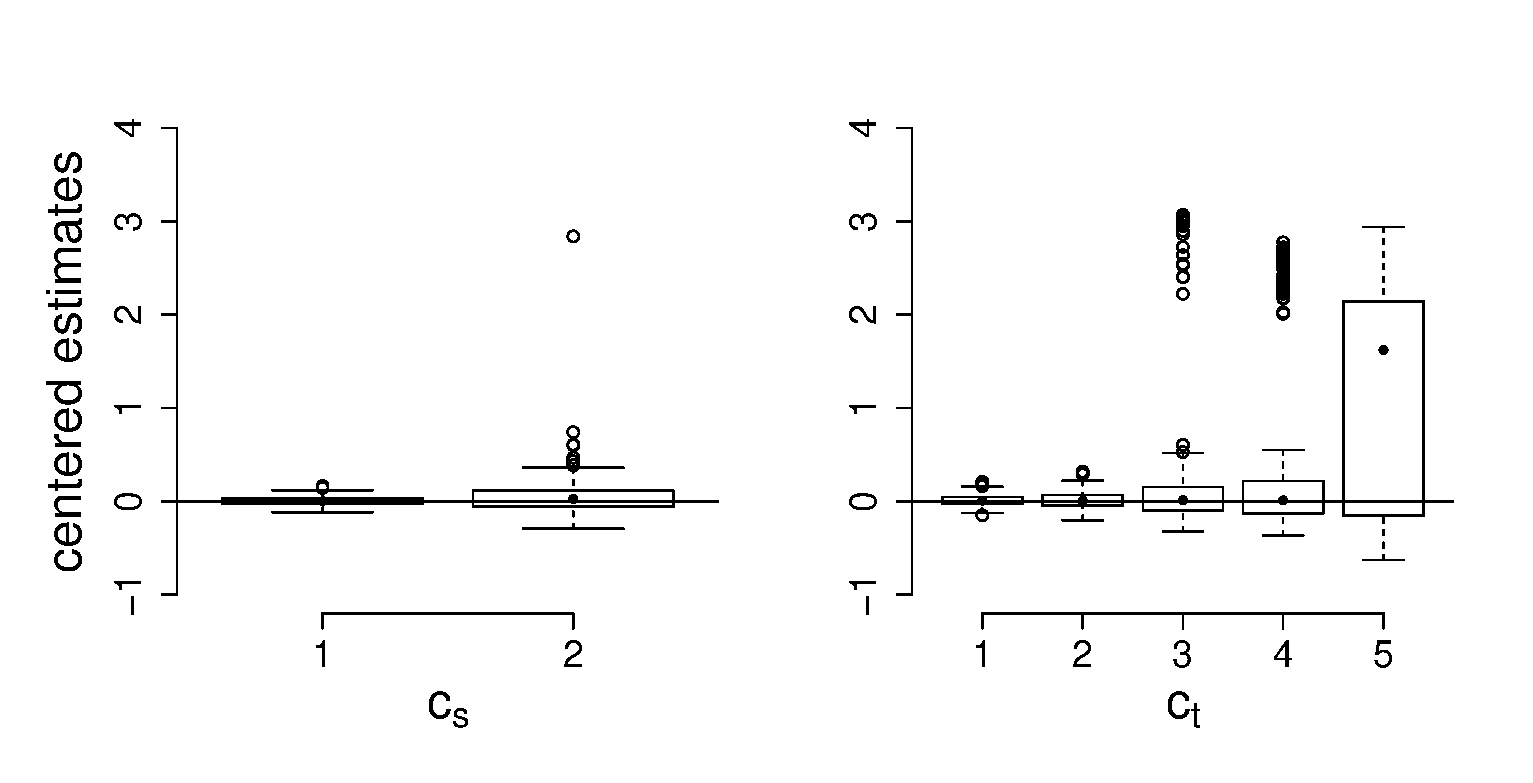
\includegraphics[scale=0.5]{em_bp}
  \caption{Shown are all $500$ estimates, centered at the true parameter values, from fitting the true model to the data generated from models $c_s,c_t$, when counts are not observed, with sample sizes small and huge, repsepectively.}
  \label{fig:em_bp}
\end{figure}

% \begin{table}
%   \centering
%   \begin{tabular}{ll|rrrr}
%     & & small & medium & large & huge \\ 
%     \hline
%     count & $c_t$ & 0.040 & 0.013 & 0.020 & 0.011 \\ 
%     & $c_s$ & 0.028 & 0.015 & 0.010 & 0.005 \\ 
%     & $c$ & 0.030 & 0.016 & 0.017 & 0.012 \\ 
%     non-count & $c_t$ & 4.151 & 3.155 & 0.941 & 1.423 \\ 
%     & $c_s$ & 0.138 & 0.096 & 0.044 & 0.032 \\ 
%     & $c$ & 2.924 & 2.078 & 0.669 & 0.547 \\ 
%   \end{tabular}
%   \caption{Max absolute bias of all $\lambda_{st}$ for each simulation scenario.}
%   \label{tab:bias}
% \end{table}

%%% Local Variables: 
%%% mode: latex
%%% TeX-master: "main"
%%% End: 

\section{Real Data}
\label{sec:data}

We analyzed a dataset that was collected to investigate the eating preferences of the wolf spider, genus \textit{Schizocosa}, towards the prey orders \textit{Diptera} and \textit{Collembola}.  Predators were collected in traps within the deciduous Berea College Forest in Madison County, Kentucky, USA and had their gut-contents analyzed to determine whether or not the spiders ate any \textit{Diptera} or \textit{Collembola} within each time period.  The left panel of figure~\ref{fig:data} plots the percentage of spiders that had the prey in their guts across time.  Prey were also collected in traps from the same area.  These data were collected for each month from October $2011$ to March $2013$.  On average, $69$ spiders, and $111$ and $297$ \textit{Diptera} and \textit{Collembola}, respectively, were caught in each time period.  The range of the sample sizes, across all $18$ months is, $11$ to $181$ for caught spiders, from $7$ to $322$ for trapped \textit{Diptera}, and from $101$ to $755$ for trapped \textit{Collembola}.  The right panel of figure~\ref{fig:data} plots the total number of each order that was caught during each time period. 

\begin{figure}
  \centering
  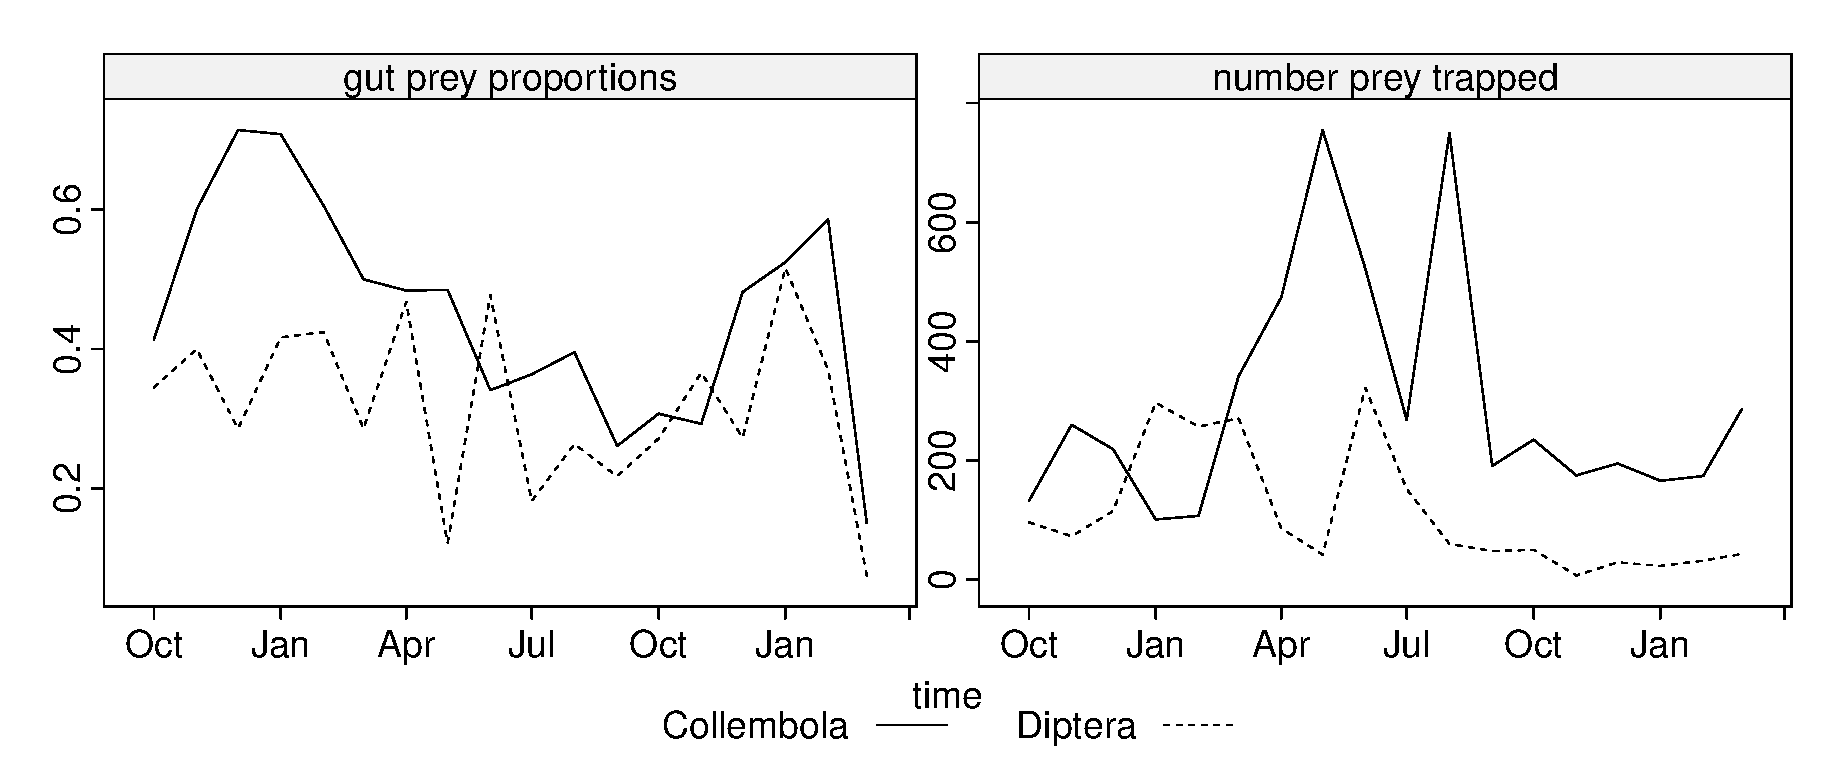
\includegraphics[scale=0.5]{data}
  \caption{For both \textit{Diptera} and \textit{Collembola}, the plots show the proportion of spiders with these orders found in their guts, and the number of these orders trapped in each time period.}
  \label{fig:data}
\end{figure}


These data provide an example of our hierarchy of hypotheses.  First, we tested model $c_{st} = c$ against $c_{st} = c_s$, to determine whether or not the wolf spider has different preferences for the two orders \textit{Diptera}  and \textit{Collembola}.  With, one degree of freedom, this likelihood ratio test indicated, $p-value < 0.0001$,  that two parameters, one for each order, fits these data better than one parameter for both.  Similarly, we tested whether or not there was a significant effect across time by testing model $c_{st} = c$ against $c_{st} = c_t$.  Here, the likelihood ratio test, with $17$ degrees of freedom, implies that the wolf spiders of the Berea College Forest eat these prey orders at different rates across the months of the year, $p-value < 0.0001$.  In fact, we find that the most parameter rich model, $\lambda_{st} = c_{st} \gamma_{st}$ fits these data better than is expected by chance, $p-value < 0.0001$.  Model $c_{st}$ estimates $72$ parameters in total; since, in this case, there are two prey of interest and $18$ time periods, it takes $36$ parameters to estimate each $c_{st}$ and $\gamma_{st}$.  Figure~\ref{fig:cst} plots the point estimates and $95\%$ confidence intervals of $c_{st}$, for both prey across all time periods.  

\begin{figure}
  \centering
  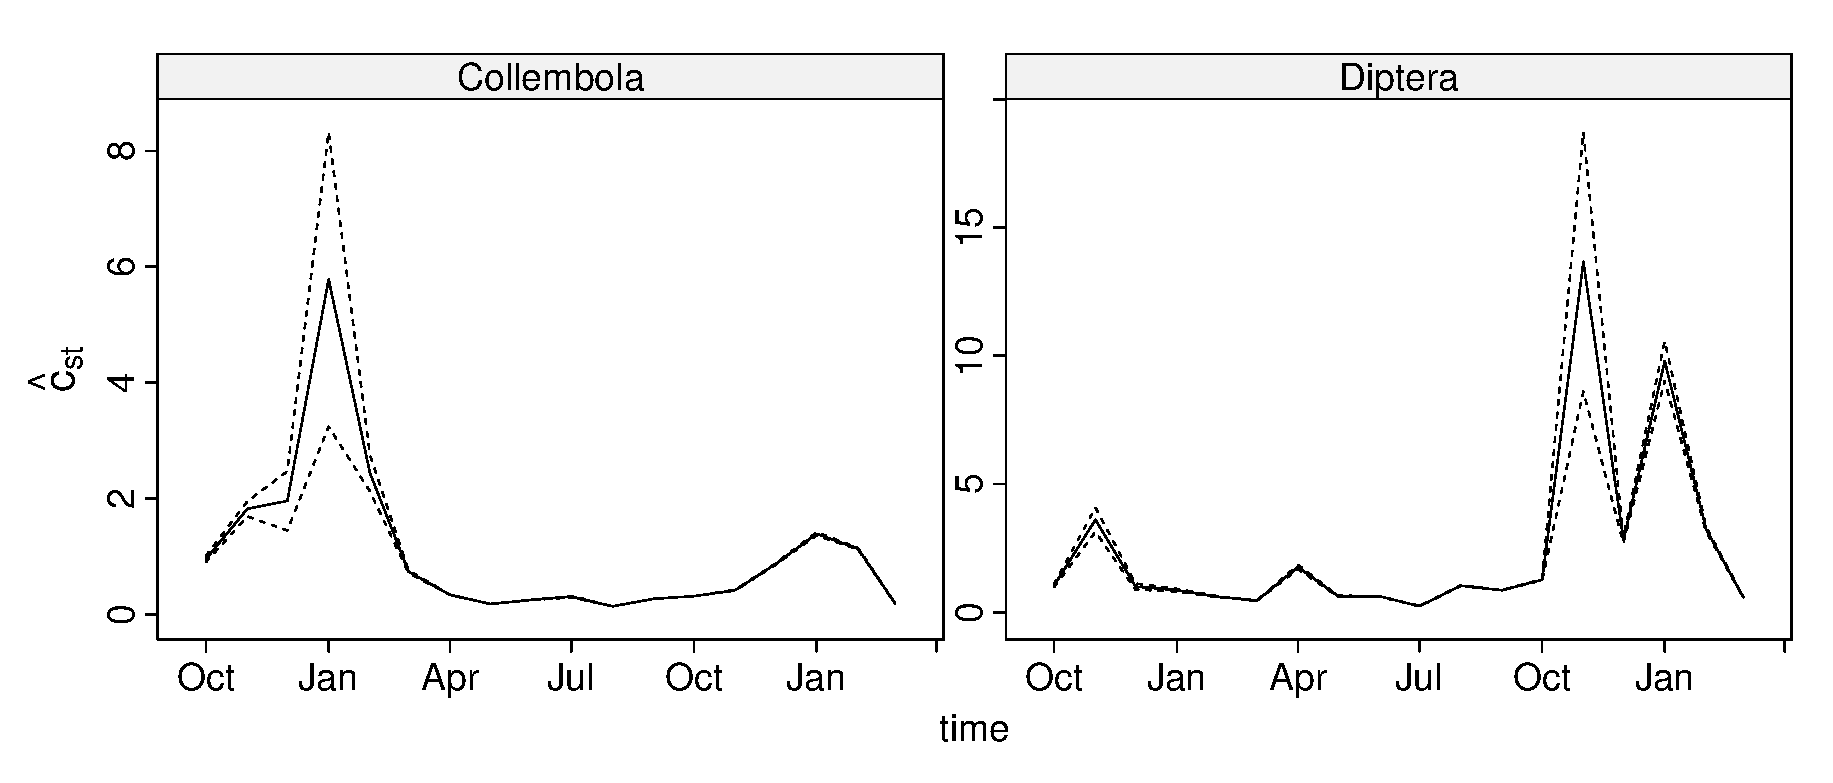
\includegraphics[scale=0.5]{cst}
  \caption{One plot for each prey order displays the point estimates and $95\%$ confidence intervals as estimated from the model $c_{st}$.}
  \label{fig:cst}
\end{figure}

With point estimates of $c_{st}$ under the model $\lambda_{st} = c_{st} \gamma_{st}$, we can test any number of linear contrasts.  For instance, $c_{1t} = c_{2t}$, for $t \in \{1, \ldots, 18\}$.  Using a level of significance of $0.05$, and after making a Bonferroni multiple comparisons adjustment, the data can not say that the two prey are differently preferred in October, November, and December of $2011$ and for March and July of $2012$.  


%%% Local Variables: 
%%% mode: latex
%%% TeX-master: "main"
%%% End: 

\section{Discussion}
\label{sec:discussion}

The model developed here allows practitioners to determine predators' preferences by testing simultaneously across an array of multiple prey species and time points.  This is achieved via a simple, but statistically powerful, likelihood ratio test.  Further testing of the ratio of rates for which predators eat to encounter prey species allows researchers to make specific conclusions about predators' preferences.  For instance, rates across time can be estimated to make statements about seasonal effects on a predator's eating habits, or relative rates across species groups allows for statements about the relative preferences for different species.

When counts of predators' gut contents are not fully observed, and instead only a binary response indicating the existence of the prey species in the gut is observed, we are able to treat the counts as missing data.  By modeling all of the observed data, both the binary responses and the number of prey species caught, and the missing count data, we are able to use the EM algorithm to extract as much information from the data as possible.  Though this is nice in theory, in practice the success of this modification to our original model is limited by the magnitude of the unknown parameters $\lambda_{st}$.  

Further developments of our model could be beneficial.  Taking into account other environmental variables that might effect a predator's eating habits, such as rain or temperature, say, might be advantageous.  

An \texttt{R} package, named \texttt{spiders}, is available on CRAN at \url{http://cran.r-project.org/web/packages/spiders/index.html} and fits all the methods discussed above.  

%%% Local Variables: 
%%% mode: latex
%%% TeX-master: "main"
%%% End: 



\bibliographystyle{plainnat}
\bibliography{refs}
\end{document}
